% Generated by script_race_tube.R with tikzDevice 0.12.6
% !TEX encoding = UTF-8 Unicode
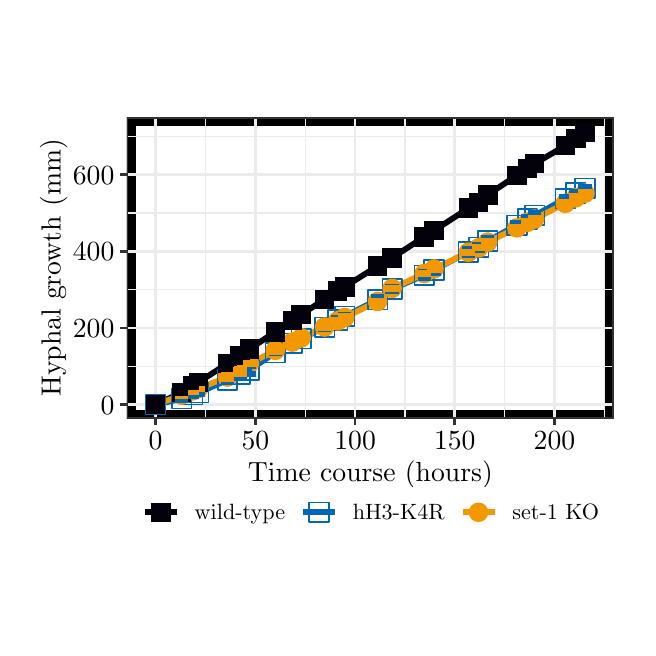
\begin{tikzpicture}[x=1pt,y=1pt]
\definecolor{fillColor}{RGB}{255,255,255}
\path[use as bounding box,fill=fillColor,fill opacity=0.00] (0,0) rectangle (216.81,216.81);
\begin{scope}
\path[clip] (  0.00, 27.42) rectangle (216.81,189.39);
\definecolor{drawColor}{RGB}{255,255,255}
\definecolor{fillColor}{RGB}{255,255,255}

\path[draw=drawColor,line width= 1.0pt,line join=round,line cap=round,fill=fillColor] (  0.00, 27.42) rectangle (216.81,189.39);
\end{scope}
\begin{scope}
\path[clip] ( 35.83, 75.62) rectangle (211.81,184.39);
\definecolor{drawColor}{RGB}{0,0,0}
\definecolor{fillColor}{RGB}{255,255,255}

\path[draw=drawColor,line width= 6.4pt,line join=round,line cap=round,fill=fillColor] ( 35.83, 75.62) rectangle (211.81,184.39);
\definecolor{drawColor}{gray}{0.92}

\path[draw=drawColor,line width= 0.5pt,line join=round] ( 35.83, 94.42) --
	(211.81, 94.42);

\path[draw=drawColor,line width= 0.5pt,line join=round] ( 35.83,122.12) --
	(211.81,122.12);

\path[draw=drawColor,line width= 0.5pt,line join=round] ( 35.83,149.83) --
	(211.81,149.83);

\path[draw=drawColor,line width= 0.5pt,line join=round] ( 35.83,177.54) --
	(211.81,177.54);

\path[draw=drawColor,line width= 0.5pt,line join=round] ( 64.27, 75.62) --
	( 64.27,184.39);

\path[draw=drawColor,line width= 0.5pt,line join=round] (100.30, 75.62) --
	(100.30,184.39);

\path[draw=drawColor,line width= 0.5pt,line join=round] (136.33, 75.62) --
	(136.33,184.39);

\path[draw=drawColor,line width= 0.5pt,line join=round] (172.36, 75.62) --
	(172.36,184.39);

\path[draw=drawColor,line width= 0.5pt,line join=round] (208.39, 75.62) --
	(208.39,184.39);

\path[draw=drawColor,line width= 1.0pt,line join=round] ( 35.83, 80.57) --
	(211.81, 80.57);

\path[draw=drawColor,line width= 1.0pt,line join=round] ( 35.83,108.27) --
	(211.81,108.27);

\path[draw=drawColor,line width= 1.0pt,line join=round] ( 35.83,135.98) --
	(211.81,135.98);

\path[draw=drawColor,line width= 1.0pt,line join=round] ( 35.83,163.68) --
	(211.81,163.68);

\path[draw=drawColor,line width= 1.0pt,line join=round] ( 46.25, 75.62) --
	( 46.25,184.39);

\path[draw=drawColor,line width= 1.0pt,line join=round] ( 82.28, 75.62) --
	( 82.28,184.39);

\path[draw=drawColor,line width= 1.0pt,line join=round] (118.31, 75.62) --
	(118.31,184.39);

\path[draw=drawColor,line width= 1.0pt,line join=round] (154.34, 75.62) --
	(154.34,184.39);

\path[draw=drawColor,line width= 1.0pt,line join=round] (190.37, 75.62) --
	(190.37,184.39);
\definecolor{drawColor}{RGB}{2,1,12}

\path[draw=drawColor,line width= 2.1pt,line join=round] ( 46.25, 80.57) --
	( 55.62, 85.02) --
	( 59.58, 87.28) --
	( 61.74, 88.65) --
	( 72.19, 95.48) --
	( 76.70, 98.37) --
	( 80.12,100.68) --
	( 89.49,106.89) --
	( 95.61,110.97) --
	( 98.86,113.17) --
	(107.29,118.64) --
	(112.02,121.63) --
	(114.56,123.19) --
	(126.44,130.64) --
	(131.70,133.67) --
	(143.31,141.22) --
	(146.81,143.48) --
	(159.27,151.57) --
	(162.94,153.65) --
	(166.23,156.42) --
	(176.79,163.46) --
	(180.61,165.98) --
	(183.17,167.66) --
	(194.28,174.17) --
	(198.05,176.76) --
	(201.39,178.88);
\definecolor{drawColor}{RGB}{0,104,183}

\path[draw=drawColor,line width= 2.1pt,line join=round] ( 46.25, 80.57) --
	( 55.62, 82.69) --
	( 59.58, 84.14) --
	( 61.74, 84.88) --
	( 72.19, 89.50) --
	( 76.70, 91.59) --
	( 80.12, 93.14) --
	( 89.49, 99.39) --
	( 95.61,102.81) --
	( 98.86,104.41) --
	(107.29,108.57) --
	(112.02,111.18) --
	(114.56,112.49) --
	(126.44,118.52) --
	(131.70,122.37) --
	(143.31,127.36) --
	(146.81,129.23) --
	(159.27,135.79) --
	(162.94,137.43) --
	(166.23,139.74) --
	(176.79,145.44) --
	(180.61,147.63) --
	(183.17,148.97) --
	(194.28,154.96) --
	(198.05,157.09) --
	(201.39,158.80);
\definecolor{drawColor}{RGB}{243,152,0}

\path[draw=drawColor,line width= 2.1pt,line join=round] ( 46.25, 80.57) --
	( 55.62, 84.01) --
	( 59.58, 85.55) --
	( 61.74, 86.43) --
	( 72.19, 90.54) --
	( 76.70, 92.53) --
	( 80.12, 95.39) --
	( 89.49,100.21) --
	( 95.61,103.17) --
	( 98.86,104.74) --
	(107.29,108.64) --
	(112.02,110.88) --
	(114.56,112.08) --
	(126.44,117.88) --
	(131.70,122.59) --
	(143.31,127.97) --
	(146.81,129.61) --
	(159.27,135.65) --
	(162.94,137.22) --
	(166.23,139.33) --
	(176.79,144.47) --
	(180.61,146.47) --
	(183.17,147.65) --
	(194.28,153.33) --
	(198.05,155.32) --
	(201.39,157.00);
\definecolor{drawColor}{RGB}{0,104,183}

\path[draw=drawColor,line width= 0.6pt,line join=round,line cap=round] ( 42.71, 77.03) rectangle ( 49.79, 84.10);

\path[draw=drawColor,line width= 0.6pt,line join=round,line cap=round] ( 52.08, 79.15) rectangle ( 59.15, 86.23);

\path[draw=drawColor,line width= 0.6pt,line join=round,line cap=round] ( 56.05, 80.61) rectangle ( 63.12, 87.68);

\path[draw=drawColor,line width= 0.6pt,line join=round,line cap=round] ( 58.21, 81.35) rectangle ( 65.28, 88.42);

\path[draw=drawColor,line width= 0.6pt,line join=round,line cap=round] ( 68.66, 85.97) rectangle ( 75.73, 93.04);

\path[draw=drawColor,line width= 0.6pt,line join=round,line cap=round] ( 73.16, 88.05) rectangle ( 80.23, 95.12);

\path[draw=drawColor,line width= 0.6pt,line join=round,line cap=round] ( 76.58, 89.61) rectangle ( 83.66, 96.68);

\path[draw=drawColor,line width= 0.6pt,line join=round,line cap=round] ( 85.95, 95.85) rectangle ( 93.02,102.92);

\path[draw=drawColor,line width= 0.6pt,line join=round,line cap=round] ( 92.08, 99.28) rectangle ( 99.15,106.35);

\path[draw=drawColor,line width= 0.6pt,line join=round,line cap=round] ( 95.32,100.87) rectangle (102.39,107.94);

\path[draw=drawColor,line width= 0.6pt,line join=round,line cap=round] (103.75,105.03) rectangle (110.82,112.10);

\path[draw=drawColor,line width= 0.6pt,line join=round,line cap=round] (108.48,107.64) rectangle (115.55,114.71);

\path[draw=drawColor,line width= 0.6pt,line join=round,line cap=round] (111.03,108.96) rectangle (118.10,116.03);

\path[draw=drawColor,line width= 0.6pt,line join=round,line cap=round] (122.91,114.98) rectangle (129.98,122.05);

\path[draw=drawColor,line width= 0.6pt,line join=round,line cap=round] (128.17,118.84) rectangle (135.24,125.91);

\path[draw=drawColor,line width= 0.6pt,line join=round,line cap=round] (139.77,123.82) rectangle (146.84,130.90);

\path[draw=drawColor,line width= 0.6pt,line join=round,line cap=round] (143.28,125.69) rectangle (150.35,132.77);

\path[draw=drawColor,line width= 0.6pt,line join=round,line cap=round] (155.73,132.25) rectangle (162.80,139.32);

\path[draw=drawColor,line width= 0.6pt,line join=round,line cap=round] (159.41,133.89) rectangle (166.48,140.96);

\path[draw=drawColor,line width= 0.6pt,line join=round,line cap=round] (162.70,136.20) rectangle (169.77,143.27);

\path[draw=drawColor,line width= 0.6pt,line join=round,line cap=round] (173.25,141.90) rectangle (180.33,148.98);

\path[draw=drawColor,line width= 0.6pt,line join=round,line cap=round] (177.07,144.10) rectangle (184.15,151.17);

\path[draw=drawColor,line width= 0.6pt,line join=round,line cap=round] (179.63,145.43) rectangle (186.70,152.51);

\path[draw=drawColor,line width= 0.6pt,line join=round,line cap=round] (190.74,151.43) rectangle (197.81,158.50);

\path[draw=drawColor,line width= 0.6pt,line join=round,line cap=round] (194.51,153.55) rectangle (201.58,160.63);

\path[draw=drawColor,line width= 0.6pt,line join=round,line cap=round] (197.85,155.26) rectangle (204.92,162.33);
\definecolor{fillColor}{RGB}{243,152,0}

\path[fill=fillColor] ( 46.25, 80.57) circle (  3.54);

\path[fill=fillColor] ( 55.62, 84.01) circle (  3.54);

\path[fill=fillColor] ( 59.58, 85.55) circle (  3.54);

\path[fill=fillColor] ( 61.74, 86.43) circle (  3.54);

\path[fill=fillColor] ( 72.19, 90.54) circle (  3.54);

\path[fill=fillColor] ( 76.70, 92.53) circle (  3.54);

\path[fill=fillColor] ( 80.12, 95.39) circle (  3.54);

\path[fill=fillColor] ( 89.49,100.21) circle (  3.54);

\path[fill=fillColor] ( 95.61,103.17) circle (  3.54);

\path[fill=fillColor] ( 98.86,104.74) circle (  3.54);

\path[fill=fillColor] (107.29,108.64) circle (  3.54);

\path[fill=fillColor] (112.02,110.88) circle (  3.54);

\path[fill=fillColor] (114.56,112.08) circle (  3.54);

\path[fill=fillColor] (126.44,117.88) circle (  3.54);

\path[fill=fillColor] (131.70,122.59) circle (  3.54);

\path[fill=fillColor] (143.31,127.97) circle (  3.54);

\path[fill=fillColor] (146.81,129.61) circle (  3.54);

\path[fill=fillColor] (159.27,135.65) circle (  3.54);

\path[fill=fillColor] (162.94,137.22) circle (  3.54);

\path[fill=fillColor] (166.23,139.33) circle (  3.54);

\path[fill=fillColor] (176.79,144.47) circle (  3.54);

\path[fill=fillColor] (180.61,146.47) circle (  3.54);

\path[fill=fillColor] (183.17,147.65) circle (  3.54);

\path[fill=fillColor] (194.28,153.33) circle (  3.54);

\path[fill=fillColor] (198.05,155.32) circle (  3.54);

\path[fill=fillColor] (201.39,157.00) circle (  3.54);
\definecolor{fillColor}{RGB}{2,1,12}

\path[fill=fillColor] ( 42.71, 77.03) --
	( 49.79, 77.03) --
	( 49.79, 84.10) --
	( 42.71, 84.10) --
	cycle;

\path[fill=fillColor] ( 52.08, 81.49) --
	( 59.15, 81.49) --
	( 59.15, 88.56) --
	( 52.08, 88.56) --
	cycle;

\path[fill=fillColor] ( 56.05, 83.75) --
	( 63.12, 83.75) --
	( 63.12, 90.82) --
	( 56.05, 90.82) --
	cycle;

\path[fill=fillColor] ( 58.21, 85.11) --
	( 65.28, 85.11) --
	( 65.28, 92.18) --
	( 58.21, 92.18) --
	cycle;

\path[fill=fillColor] ( 68.66, 91.94) --
	( 75.73, 91.94) --
	( 75.73, 99.02) --
	( 68.66, 99.02) --
	cycle;

\path[fill=fillColor] ( 73.16, 94.83) --
	( 80.23, 94.83) --
	( 80.23,101.90) --
	( 73.16,101.90) --
	cycle;

\path[fill=fillColor] ( 76.58, 97.14) --
	( 83.66, 97.14) --
	( 83.66,104.21) --
	( 76.58,104.21) --
	cycle;

\path[fill=fillColor] ( 85.95,103.35) --
	( 93.02,103.35) --
	( 93.02,110.42) --
	( 85.95,110.42) --
	cycle;

\path[fill=fillColor] ( 92.08,107.44) --
	( 99.15,107.44) --
	( 99.15,114.51) --
	( 92.08,114.51) --
	cycle;

\path[fill=fillColor] ( 95.32,109.63) --
	(102.39,109.63) --
	(102.39,116.70) --
	( 95.32,116.70) --
	cycle;

\path[fill=fillColor] (103.75,115.10) --
	(110.82,115.10) --
	(110.82,122.17) --
	(103.75,122.17) --
	cycle;

\path[fill=fillColor] (108.48,118.09) --
	(115.55,118.09) --
	(115.55,125.17) --
	(108.48,125.17) --
	cycle;

\path[fill=fillColor] (111.03,119.65) --
	(118.10,119.65) --
	(118.10,126.72) --
	(111.03,126.72) --
	cycle;

\path[fill=fillColor] (122.91,127.11) --
	(129.98,127.11) --
	(129.98,134.18) --
	(122.91,134.18) --
	cycle;

\path[fill=fillColor] (128.17,130.13) --
	(135.24,130.13) --
	(135.24,137.20) --
	(128.17,137.20) --
	cycle;

\path[fill=fillColor] (139.77,137.68) --
	(146.84,137.68) --
	(146.84,144.75) --
	(139.77,144.75) --
	cycle;

\path[fill=fillColor] (143.28,139.94) --
	(150.35,139.94) --
	(150.35,147.02) --
	(143.28,147.02) --
	cycle;

\path[fill=fillColor] (155.73,148.03) --
	(162.80,148.03) --
	(162.80,155.11) --
	(155.73,155.11) --
	cycle;

\path[fill=fillColor] (159.41,150.11) --
	(166.48,150.11) --
	(166.48,157.19) --
	(159.41,157.19) --
	cycle;

\path[fill=fillColor] (162.70,152.88) --
	(169.77,152.88) --
	(169.77,159.96) --
	(162.70,159.96) --
	cycle;

\path[fill=fillColor] (173.25,159.92) --
	(180.33,159.92) --
	(180.33,167.00) --
	(173.25,167.00) --
	cycle;

\path[fill=fillColor] (177.07,162.44) --
	(184.15,162.44) --
	(184.15,169.51) --
	(177.07,169.51) --
	cycle;

\path[fill=fillColor] (179.63,164.13) --
	(186.70,164.13) --
	(186.70,171.20) --
	(179.63,171.20) --
	cycle;

\path[fill=fillColor] (190.74,170.64) --
	(197.81,170.64) --
	(197.81,177.71) --
	(190.74,177.71) --
	cycle;

\path[fill=fillColor] (194.51,173.22) --
	(201.58,173.22) --
	(201.58,180.30) --
	(194.51,180.30) --
	cycle;

\path[fill=fillColor] (197.85,175.35) --
	(204.92,175.35) --
	(204.92,182.42) --
	(197.85,182.42) --
	cycle;

\path[draw=drawColor,line width= 2.1pt,line join=round] ( 43.83, 80.57) --
	( 48.67, 80.57);

\path[draw=drawColor,line width= 2.1pt,line join=round] ( 46.25, 80.57) --
	( 46.25, 80.57);

\path[draw=drawColor,line width= 2.1pt,line join=round] ( 43.83, 80.57) --
	( 48.67, 80.57);

\path[draw=drawColor,line width= 2.1pt,line join=round] ( 53.19, 83.03) --
	( 58.04, 83.03);

\path[draw=drawColor,line width= 2.1pt,line join=round] ( 55.62, 83.03) --
	( 55.62, 82.36);

\path[draw=drawColor,line width= 2.1pt,line join=round] ( 53.19, 82.36) --
	( 58.04, 82.36);

\path[draw=drawColor,line width= 2.1pt,line join=round] ( 57.16, 84.59) --
	( 62.01, 84.59);

\path[draw=drawColor,line width= 2.1pt,line join=round] ( 59.58, 84.59) --
	( 59.58, 83.70);

\path[draw=drawColor,line width= 2.1pt,line join=round] ( 57.16, 83.70) --
	( 62.01, 83.70);

\path[draw=drawColor,line width= 2.1pt,line join=round] ( 59.32, 85.40) --
	( 64.17, 85.40);

\path[draw=drawColor,line width= 2.1pt,line join=round] ( 61.74, 85.40) --
	( 61.74, 84.37);

\path[draw=drawColor,line width= 2.1pt,line join=round] ( 59.32, 84.37) --
	( 64.17, 84.37);

\path[draw=drawColor,line width= 2.1pt,line join=round] ( 69.77, 90.41) --
	( 74.62, 90.41);

\path[draw=drawColor,line width= 2.1pt,line join=round] ( 72.19, 90.41) --
	( 72.19, 88.60);

\path[draw=drawColor,line width= 2.1pt,line join=round] ( 69.77, 88.60) --
	( 74.62, 88.60);

\path[draw=drawColor,line width= 2.1pt,line join=round] ( 74.27, 92.85) --
	( 79.12, 92.85);

\path[draw=drawColor,line width= 2.1pt,line join=round] ( 76.70, 92.85) --
	( 76.70, 90.33);

\path[draw=drawColor,line width= 2.1pt,line join=round] ( 74.27, 90.33) --
	( 79.12, 90.33);

\path[draw=drawColor,line width= 2.1pt,line join=round] ( 77.70, 94.54) --
	( 82.54, 94.54);

\path[draw=drawColor,line width= 2.1pt,line join=round] ( 80.12, 94.54) --
	( 80.12, 91.75);

\path[draw=drawColor,line width= 2.1pt,line join=round] ( 77.70, 91.75) --
	( 82.54, 91.75);

\path[draw=drawColor,line width= 2.1pt,line join=round] ( 87.06, 99.54) --
	( 91.91, 99.54);

\path[draw=drawColor,line width= 2.1pt,line join=round] ( 89.49, 99.54) --
	( 89.49, 99.23);

\path[draw=drawColor,line width= 2.1pt,line join=round] ( 87.06, 99.23) --
	( 91.91, 99.23);

\path[draw=drawColor,line width= 2.1pt,line join=round] ( 93.19,102.93) --
	( 98.04,102.93);

\path[draw=drawColor,line width= 2.1pt,line join=round] ( 95.61,102.93) --
	( 95.61,102.70);

\path[draw=drawColor,line width= 2.1pt,line join=round] ( 93.19,102.70) --
	( 98.04,102.70);

\path[draw=drawColor,line width= 2.1pt,line join=round] ( 96.43,104.61) --
	(101.28,104.61);

\path[draw=drawColor,line width= 2.1pt,line join=round] ( 98.86,104.61) --
	( 98.86,104.21);

\path[draw=drawColor,line width= 2.1pt,line join=round] ( 96.43,104.21) --
	(101.28,104.21);

\path[draw=drawColor,line width= 2.1pt,line join=round] (104.86,109.09) --
	(109.71,109.09);

\path[draw=drawColor,line width= 2.1pt,line join=round] (107.29,109.09) --
	(107.29,108.05);

\path[draw=drawColor,line width= 2.1pt,line join=round] (104.86,108.05) --
	(109.71,108.05);

\path[draw=drawColor,line width= 2.1pt,line join=round] (109.59,111.76) --
	(114.44,111.76);

\path[draw=drawColor,line width= 2.1pt,line join=round] (112.02,111.76) --
	(112.02,110.59);

\path[draw=drawColor,line width= 2.1pt,line join=round] (109.59,110.59) --
	(114.44,110.59);

\path[draw=drawColor,line width= 2.1pt,line join=round] (112.14,113.18) --
	(116.99,113.18);

\path[draw=drawColor,line width= 2.1pt,line join=round] (114.56,113.18) --
	(114.56,111.80);

\path[draw=drawColor,line width= 2.1pt,line join=round] (112.14,111.80) --
	(116.99,111.80);

\path[draw=drawColor,line width= 2.1pt,line join=round] (124.02,119.42) --
	(128.87,119.42);

\path[draw=drawColor,line width= 2.1pt,line join=round] (126.44,119.42) --
	(126.44,117.62);

\path[draw=drawColor,line width= 2.1pt,line join=round] (124.02,117.62) --
	(128.87,117.62);

\path[draw=drawColor,line width= 2.1pt,line join=round] (129.28,123.25) --
	(134.13,123.25);

\path[draw=drawColor,line width= 2.1pt,line join=round] (131.70,123.25) --
	(131.70,121.49);

\path[draw=drawColor,line width= 2.1pt,line join=round] (129.28,121.49) --
	(134.13,121.49);

\path[draw=drawColor,line width= 2.1pt,line join=round] (140.88,128.43) --
	(145.73,128.43);

\path[draw=drawColor,line width= 2.1pt,line join=round] (143.31,128.43) --
	(143.31,126.29);

\path[draw=drawColor,line width= 2.1pt,line join=round] (140.88,126.29) --
	(145.73,126.29);

\path[draw=drawColor,line width= 2.1pt,line join=round] (144.39,130.17) --
	(149.24,130.17);

\path[draw=drawColor,line width= 2.1pt,line join=round] (146.81,130.17) --
	(146.81,128.29);

\path[draw=drawColor,line width= 2.1pt,line join=round] (144.39,128.29) --
	(149.24,128.29);

\path[draw=drawColor,line width= 2.1pt,line join=round] (156.84,136.77) --
	(161.69,136.77);

\path[draw=drawColor,line width= 2.1pt,line join=round] (159.27,136.77) --
	(159.27,134.81);

\path[draw=drawColor,line width= 2.1pt,line join=round] (156.84,134.81) --
	(161.69,134.81);

\path[draw=drawColor,line width= 2.1pt,line join=round] (160.52,138.34) --
	(165.37,138.34);

\path[draw=drawColor,line width= 2.1pt,line join=round] (162.94,138.34) --
	(162.94,136.52);

\path[draw=drawColor,line width= 2.1pt,line join=round] (160.52,136.52) --
	(165.37,136.52);

\path[draw=drawColor,line width= 2.1pt,line join=round] (163.81,140.68) --
	(168.66,140.68);

\path[draw=drawColor,line width= 2.1pt,line join=round] (166.23,140.68) --
	(166.23,138.79);

\path[draw=drawColor,line width= 2.1pt,line join=round] (163.81,138.79) --
	(168.66,138.79);

\path[draw=drawColor,line width= 2.1pt,line join=round] (174.37,146.21) --
	(179.21,146.21);

\path[draw=drawColor,line width= 2.1pt,line join=round] (176.79,146.21) --
	(176.79,144.66);

\path[draw=drawColor,line width= 2.1pt,line join=round] (174.37,144.66) --
	(179.21,144.66);

\path[draw=drawColor,line width= 2.1pt,line join=round] (178.19,148.39) --
	(183.03,148.39);

\path[draw=drawColor,line width= 2.1pt,line join=round] (180.61,148.39) --
	(180.61,146.88);

\path[draw=drawColor,line width= 2.1pt,line join=round] (178.19,146.88) --
	(183.03,146.88);

\path[draw=drawColor,line width= 2.1pt,line join=round] (180.74,149.73) --
	(185.59,149.73);

\path[draw=drawColor,line width= 2.1pt,line join=round] (183.17,149.73) --
	(183.17,148.21);

\path[draw=drawColor,line width= 2.1pt,line join=round] (180.74,148.21) --
	(185.59,148.21);

\path[draw=drawColor,line width= 2.1pt,line join=round] (191.85,155.56) --
	(196.70,155.56);

\path[draw=drawColor,line width= 2.1pt,line join=round] (194.28,155.56) --
	(194.28,154.37);

\path[draw=drawColor,line width= 2.1pt,line join=round] (191.85,154.37) --
	(196.70,154.37);

\path[draw=drawColor,line width= 2.1pt,line join=round] (195.62,157.62) --
	(200.47,157.62);

\path[draw=drawColor,line width= 2.1pt,line join=round] (198.05,157.62) --
	(198.05,156.56);

\path[draw=drawColor,line width= 2.1pt,line join=round] (195.62,156.56) --
	(200.47,156.56);

\path[draw=drawColor,line width= 2.1pt,line join=round] (198.96,159.30) --
	(203.81,159.30);

\path[draw=drawColor,line width= 2.1pt,line join=round] (201.39,159.30) --
	(201.39,158.29);

\path[draw=drawColor,line width= 2.1pt,line join=round] (198.96,158.29) --
	(203.81,158.29);
\definecolor{drawColor}{RGB}{243,152,0}

\path[draw=drawColor,line width= 2.1pt,line join=round] ( 43.83, 80.57) --
	( 48.67, 80.57);

\path[draw=drawColor,line width= 2.1pt,line join=round] ( 46.25, 80.57) --
	( 46.25, 80.57);

\path[draw=drawColor,line width= 2.1pt,line join=round] ( 43.83, 80.57) --
	( 48.67, 80.57);

\path[draw=drawColor,line width= 2.1pt,line join=round] ( 53.19, 84.17) --
	( 58.04, 84.17);

\path[draw=drawColor,line width= 2.1pt,line join=round] ( 55.62, 84.17) --
	( 55.62, 83.84);

\path[draw=drawColor,line width= 2.1pt,line join=round] ( 53.19, 83.84) --
	( 58.04, 83.84);

\path[draw=drawColor,line width= 2.1pt,line join=round] ( 57.16, 85.88) --
	( 62.01, 85.88);

\path[draw=drawColor,line width= 2.1pt,line join=round] ( 59.58, 85.88) --
	( 59.58, 85.23);

\path[draw=drawColor,line width= 2.1pt,line join=round] ( 57.16, 85.23) --
	( 62.01, 85.23);

\path[draw=drawColor,line width= 2.1pt,line join=round] ( 59.32, 86.83) --
	( 64.17, 86.83);

\path[draw=drawColor,line width= 2.1pt,line join=round] ( 61.74, 86.83) --
	( 61.74, 86.03);

\path[draw=drawColor,line width= 2.1pt,line join=round] ( 59.32, 86.03) --
	( 64.17, 86.03);

\path[draw=drawColor,line width= 2.1pt,line join=round] ( 69.77, 91.17) --
	( 74.62, 91.17);

\path[draw=drawColor,line width= 2.1pt,line join=round] ( 72.19, 91.17) --
	( 72.19, 89.91);

\path[draw=drawColor,line width= 2.1pt,line join=round] ( 69.77, 89.91) --
	( 74.62, 89.91);

\path[draw=drawColor,line width= 2.1pt,line join=round] ( 74.27, 93.41) --
	( 79.12, 93.41);

\path[draw=drawColor,line width= 2.1pt,line join=round] ( 76.70, 93.41) --
	( 76.70, 91.64);

\path[draw=drawColor,line width= 2.1pt,line join=round] ( 74.27, 91.64) --
	( 79.12, 91.64);

\path[draw=drawColor,line width= 2.1pt,line join=round] ( 77.70, 95.67) --
	( 82.54, 95.67);

\path[draw=drawColor,line width= 2.1pt,line join=round] ( 80.12, 95.67) --
	( 80.12, 95.11);

\path[draw=drawColor,line width= 2.1pt,line join=round] ( 77.70, 95.11) --
	( 82.54, 95.11);

\path[draw=drawColor,line width= 2.1pt,line join=round] ( 87.06,100.67) --
	( 91.91,100.67);

\path[draw=drawColor,line width= 2.1pt,line join=round] ( 89.49,100.67) --
	( 89.49, 99.75);

\path[draw=drawColor,line width= 2.1pt,line join=round] ( 87.06, 99.75) --
	( 91.91, 99.75);

\path[draw=drawColor,line width= 2.1pt,line join=round] ( 93.19,103.57) --
	( 98.04,103.57);

\path[draw=drawColor,line width= 2.1pt,line join=round] ( 95.61,103.57) --
	( 95.61,102.77);

\path[draw=drawColor,line width= 2.1pt,line join=round] ( 93.19,102.77) --
	( 98.04,102.77);

\path[draw=drawColor,line width= 2.1pt,line join=round] ( 96.43,105.09) --
	(101.28,105.09);

\path[draw=drawColor,line width= 2.1pt,line join=round] ( 98.86,105.09) --
	( 98.86,104.39);

\path[draw=drawColor,line width= 2.1pt,line join=round] ( 96.43,104.39) --
	(101.28,104.39);

\path[draw=drawColor,line width= 2.1pt,line join=round] (104.86,109.04) --
	(109.71,109.04);

\path[draw=drawColor,line width= 2.1pt,line join=round] (107.29,109.04) --
	(107.29,108.25);

\path[draw=drawColor,line width= 2.1pt,line join=round] (104.86,108.25) --
	(109.71,108.25);

\path[draw=drawColor,line width= 2.1pt,line join=round] (109.59,111.30) --
	(114.44,111.30);

\path[draw=drawColor,line width= 2.1pt,line join=round] (112.02,111.30) --
	(112.02,110.46);

\path[draw=drawColor,line width= 2.1pt,line join=round] (109.59,110.46) --
	(114.44,110.46);

\path[draw=drawColor,line width= 2.1pt,line join=round] (112.14,112.50) --
	(116.99,112.50);

\path[draw=drawColor,line width= 2.1pt,line join=round] (114.56,112.50) --
	(114.56,111.66);

\path[draw=drawColor,line width= 2.1pt,line join=round] (112.14,111.66) --
	(116.99,111.66);

\path[draw=drawColor,line width= 2.1pt,line join=round] (124.02,118.19) --
	(128.87,118.19);

\path[draw=drawColor,line width= 2.1pt,line join=round] (126.44,118.19) --
	(126.44,117.57);

\path[draw=drawColor,line width= 2.1pt,line join=round] (124.02,117.57) --
	(128.87,117.57);

\path[draw=drawColor,line width= 2.1pt,line join=round] (129.28,122.90) --
	(134.13,122.90);

\path[draw=drawColor,line width= 2.1pt,line join=round] (131.70,122.90) --
	(131.70,122.28);

\path[draw=drawColor,line width= 2.1pt,line join=round] (129.28,122.28) --
	(134.13,122.28);

\path[draw=drawColor,line width= 2.1pt,line join=round] (140.88,128.33) --
	(145.73,128.33);

\path[draw=drawColor,line width= 2.1pt,line join=round] (143.31,128.33) --
	(143.31,127.60);

\path[draw=drawColor,line width= 2.1pt,line join=round] (140.88,127.60) --
	(145.73,127.60);

\path[draw=drawColor,line width= 2.1pt,line join=round] (144.39,129.88) --
	(149.24,129.88);

\path[draw=drawColor,line width= 2.1pt,line join=round] (146.81,129.88) --
	(146.81,129.33);

\path[draw=drawColor,line width= 2.1pt,line join=round] (144.39,129.33) --
	(149.24,129.33);

\path[draw=drawColor,line width= 2.1pt,line join=round] (156.84,135.96) --
	(161.69,135.96);

\path[draw=drawColor,line width= 2.1pt,line join=round] (159.27,135.96) --
	(159.27,135.35);

\path[draw=drawColor,line width= 2.1pt,line join=round] (156.84,135.35) --
	(161.69,135.35);

\path[draw=drawColor,line width= 2.1pt,line join=round] (160.52,137.44) --
	(165.37,137.44);

\path[draw=drawColor,line width= 2.1pt,line join=round] (162.94,137.44) --
	(162.94,137.01);

\path[draw=drawColor,line width= 2.1pt,line join=round] (160.52,137.01) --
	(165.37,137.01);

\path[draw=drawColor,line width= 2.1pt,line join=round] (163.81,139.58) --
	(168.66,139.58);

\path[draw=drawColor,line width= 2.1pt,line join=round] (166.23,139.58) --
	(166.23,139.07);

\path[draw=drawColor,line width= 2.1pt,line join=round] (163.81,139.07) --
	(168.66,139.07);

\path[draw=drawColor,line width= 2.1pt,line join=round] (174.37,144.84) --
	(179.21,144.84);

\path[draw=drawColor,line width= 2.1pt,line join=round] (176.79,144.84) --
	(176.79,144.11);

\path[draw=drawColor,line width= 2.1pt,line join=round] (174.37,144.11) --
	(179.21,144.11);

\path[draw=drawColor,line width= 2.1pt,line join=round] (178.19,146.87) --
	(183.03,146.87);

\path[draw=drawColor,line width= 2.1pt,line join=round] (180.61,146.87) --
	(180.61,146.08);

\path[draw=drawColor,line width= 2.1pt,line join=round] (178.19,146.08) --
	(183.03,146.08);

\path[draw=drawColor,line width= 2.1pt,line join=round] (180.74,148.03) --
	(185.59,148.03);

\path[draw=drawColor,line width= 2.1pt,line join=round] (183.17,148.03) --
	(183.17,147.27);

\path[draw=drawColor,line width= 2.1pt,line join=round] (180.74,147.27) --
	(185.59,147.27);

\path[draw=drawColor,line width= 2.1pt,line join=round] (191.85,153.92) --
	(196.70,153.92);

\path[draw=drawColor,line width= 2.1pt,line join=round] (194.28,153.92) --
	(194.28,152.74);

\path[draw=drawColor,line width= 2.1pt,line join=round] (191.85,152.74) --
	(196.70,152.74);

\path[draw=drawColor,line width= 2.1pt,line join=round] (195.62,155.89) --
	(200.47,155.89);

\path[draw=drawColor,line width= 2.1pt,line join=round] (198.05,155.89) --
	(198.05,154.75);

\path[draw=drawColor,line width= 2.1pt,line join=round] (195.62,154.75) --
	(200.47,154.75);

\path[draw=drawColor,line width= 2.1pt,line join=round] (198.96,157.63) --
	(203.81,157.63);

\path[draw=drawColor,line width= 2.1pt,line join=round] (201.39,157.63) --
	(201.39,156.37);

\path[draw=drawColor,line width= 2.1pt,line join=round] (198.96,156.37) --
	(203.81,156.37);
\definecolor{drawColor}{RGB}{2,1,12}

\path[draw=drawColor,line width= 2.1pt,line join=round] ( 43.83, 80.57) --
	( 48.67, 80.57);

\path[draw=drawColor,line width= 2.1pt,line join=round] ( 46.25, 80.57) --
	( 46.25, 80.57);

\path[draw=drawColor,line width= 2.1pt,line join=round] ( 43.83, 80.57) --
	( 48.67, 80.57);

\path[draw=drawColor,line width= 2.1pt,line join=round] ( 53.19, 85.15) --
	( 58.04, 85.15);

\path[draw=drawColor,line width= 2.1pt,line join=round] ( 55.62, 85.15) --
	( 55.62, 84.89);

\path[draw=drawColor,line width= 2.1pt,line join=round] ( 53.19, 84.89) --
	( 58.04, 84.89);

\path[draw=drawColor,line width= 2.1pt,line join=round] ( 57.16, 87.51) --
	( 62.01, 87.51);

\path[draw=drawColor,line width= 2.1pt,line join=round] ( 59.58, 87.51) --
	( 59.58, 87.06);

\path[draw=drawColor,line width= 2.1pt,line join=round] ( 57.16, 87.06) --
	( 62.01, 87.06);

\path[draw=drawColor,line width= 2.1pt,line join=round] ( 59.32, 88.90) --
	( 64.17, 88.90);

\path[draw=drawColor,line width= 2.1pt,line join=round] ( 61.74, 88.90) --
	( 61.74, 88.39);

\path[draw=drawColor,line width= 2.1pt,line join=round] ( 59.32, 88.39) --
	( 64.17, 88.39);

\path[draw=drawColor,line width= 2.1pt,line join=round] ( 69.77, 95.88) --
	( 74.62, 95.88);

\path[draw=drawColor,line width= 2.1pt,line join=round] ( 72.19, 95.88) --
	( 72.19, 95.08);

\path[draw=drawColor,line width= 2.1pt,line join=round] ( 69.77, 95.08) --
	( 74.62, 95.08);

\path[draw=drawColor,line width= 2.1pt,line join=round] ( 74.27, 98.71) --
	( 79.12, 98.71);

\path[draw=drawColor,line width= 2.1pt,line join=round] ( 76.70, 98.71) --
	( 76.70, 98.03);

\path[draw=drawColor,line width= 2.1pt,line join=round] ( 74.27, 98.03) --
	( 79.12, 98.03);

\path[draw=drawColor,line width= 2.1pt,line join=round] ( 77.70,101.03) --
	( 82.54,101.03);

\path[draw=drawColor,line width= 2.1pt,line join=round] ( 80.12,101.03) --
	( 80.12,100.33);

\path[draw=drawColor,line width= 2.1pt,line join=round] ( 77.70,100.33) --
	( 82.54,100.33);

\path[draw=drawColor,line width= 2.1pt,line join=round] ( 87.06,107.37) --
	( 91.91,107.37);

\path[draw=drawColor,line width= 2.1pt,line join=round] ( 89.49,107.37) --
	( 89.49,106.40);

\path[draw=drawColor,line width= 2.1pt,line join=round] ( 87.06,106.40) --
	( 91.91,106.40);

\path[draw=drawColor,line width= 2.1pt,line join=round] ( 93.19,111.46) --
	( 98.04,111.46);

\path[draw=drawColor,line width= 2.1pt,line join=round] ( 95.61,111.46) --
	( 95.61,110.49);

\path[draw=drawColor,line width= 2.1pt,line join=round] ( 93.19,110.49) --
	( 98.04,110.49);

\path[draw=drawColor,line width= 2.1pt,line join=round] ( 96.43,113.56) --
	(101.28,113.56);

\path[draw=drawColor,line width= 2.1pt,line join=round] ( 98.86,113.56) --
	( 98.86,112.77);

\path[draw=drawColor,line width= 2.1pt,line join=round] ( 96.43,112.77) --
	(101.28,112.77);

\path[draw=drawColor,line width= 2.1pt,line join=round] (104.86,119.04) --
	(109.71,119.04);

\path[draw=drawColor,line width= 2.1pt,line join=round] (107.29,119.04) --
	(107.29,118.24);

\path[draw=drawColor,line width= 2.1pt,line join=round] (104.86,118.24) --
	(109.71,118.24);

\path[draw=drawColor,line width= 2.1pt,line join=round] (109.59,122.05) --
	(114.44,122.05);

\path[draw=drawColor,line width= 2.1pt,line join=round] (112.02,122.05) --
	(112.02,121.21);

\path[draw=drawColor,line width= 2.1pt,line join=round] (109.59,121.21) --
	(114.44,121.21);

\path[draw=drawColor,line width= 2.1pt,line join=round] (112.14,123.55) --
	(116.99,123.55);

\path[draw=drawColor,line width= 2.1pt,line join=round] (114.56,123.55) --
	(114.56,122.82);

\path[draw=drawColor,line width= 2.1pt,line join=round] (112.14,122.82) --
	(116.99,122.82);

\path[draw=drawColor,line width= 2.1pt,line join=round] (124.02,130.85) --
	(128.87,130.85);

\path[draw=drawColor,line width= 2.1pt,line join=round] (126.44,130.85) --
	(126.44,130.44);

\path[draw=drawColor,line width= 2.1pt,line join=round] (124.02,130.44) --
	(128.87,130.44);

\path[draw=drawColor,line width= 2.1pt,line join=round] (129.28,134.40) --
	(134.13,134.40);

\path[draw=drawColor,line width= 2.1pt,line join=round] (131.70,134.40) --
	(131.70,132.94);

\path[draw=drawColor,line width= 2.1pt,line join=round] (129.28,132.94) --
	(134.13,132.94);

\path[draw=drawColor,line width= 2.1pt,line join=round] (140.88,141.76) --
	(145.73,141.76);

\path[draw=drawColor,line width= 2.1pt,line join=round] (143.31,141.76) --
	(143.31,140.68);

\path[draw=drawColor,line width= 2.1pt,line join=round] (140.88,140.68) --
	(145.73,140.68);

\path[draw=drawColor,line width= 2.1pt,line join=round] (144.39,144.05) --
	(149.24,144.05);

\path[draw=drawColor,line width= 2.1pt,line join=round] (146.81,144.05) --
	(146.81,142.91);

\path[draw=drawColor,line width= 2.1pt,line join=round] (144.39,142.91) --
	(149.24,142.91);

\path[draw=drawColor,line width= 2.1pt,line join=round] (156.84,152.05) --
	(161.69,152.05);

\path[draw=drawColor,line width= 2.1pt,line join=round] (159.27,152.05) --
	(159.27,151.09);

\path[draw=drawColor,line width= 2.1pt,line join=round] (156.84,151.09) --
	(161.69,151.09);

\path[draw=drawColor,line width= 2.1pt,line join=round] (160.52,154.14) --
	(165.37,154.14);

\path[draw=drawColor,line width= 2.1pt,line join=round] (162.94,154.14) --
	(162.94,153.16);

\path[draw=drawColor,line width= 2.1pt,line join=round] (160.52,153.16) --
	(165.37,153.16);

\path[draw=drawColor,line width= 2.1pt,line join=round] (163.81,156.97) --
	(168.66,156.97);

\path[draw=drawColor,line width= 2.1pt,line join=round] (166.23,156.97) --
	(166.23,155.87);

\path[draw=drawColor,line width= 2.1pt,line join=round] (163.81,155.87) --
	(168.66,155.87);

\path[draw=drawColor,line width= 2.1pt,line join=round] (174.37,164.09) --
	(179.21,164.09);

\path[draw=drawColor,line width= 2.1pt,line join=round] (176.79,164.09) --
	(176.79,162.84);

\path[draw=drawColor,line width= 2.1pt,line join=round] (174.37,162.84) --
	(179.21,162.84);

\path[draw=drawColor,line width= 2.1pt,line join=round] (178.19,166.72) --
	(183.03,166.72);

\path[draw=drawColor,line width= 2.1pt,line join=round] (180.61,166.72) --
	(180.61,165.23);

\path[draw=drawColor,line width= 2.1pt,line join=round] (178.19,165.23) --
	(183.03,165.23);

\path[draw=drawColor,line width= 2.1pt,line join=round] (180.74,168.38) --
	(185.59,168.38);

\path[draw=drawColor,line width= 2.1pt,line join=round] (183.17,168.38) --
	(183.17,166.94);

\path[draw=drawColor,line width= 2.1pt,line join=round] (180.74,166.94) --
	(185.59,166.94);

\path[draw=drawColor,line width= 2.1pt,line join=round] (191.85,174.56) --
	(196.70,174.56);

\path[draw=drawColor,line width= 2.1pt,line join=round] (194.28,174.56) --
	(194.28,173.79);

\path[draw=drawColor,line width= 2.1pt,line join=round] (191.85,173.79) --
	(196.70,173.79);

\path[draw=drawColor,line width= 2.1pt,line join=round] (195.62,177.12) --
	(200.47,177.12);

\path[draw=drawColor,line width= 2.1pt,line join=round] (198.05,177.12) --
	(198.05,176.40);

\path[draw=drawColor,line width= 2.1pt,line join=round] (195.62,176.40) --
	(200.47,176.40);

\path[draw=drawColor,line width= 2.1pt,line join=round] (198.96,179.44) --
	(203.81,179.44);

\path[draw=drawColor,line width= 2.1pt,line join=round] (201.39,179.44) --
	(201.39,178.33);

\path[draw=drawColor,line width= 2.1pt,line join=round] (198.96,178.33) --
	(203.81,178.33);
\definecolor{drawColor}{gray}{0.20}

\path[draw=drawColor,line width= 1.0pt,line join=round,line cap=round] ( 35.83, 75.62) rectangle (211.81,184.39);
\end{scope}
\begin{scope}
\path[clip] (  0.00,  0.00) rectangle (216.81,216.81);
\definecolor{drawColor}{RGB}{0,0,0}

\node[text=drawColor,anchor=base east,inner sep=0pt, outer sep=0pt, scale=  1.00] at ( 31.33, 77.12) {0};

\node[text=drawColor,anchor=base east,inner sep=0pt, outer sep=0pt, scale=  1.00] at ( 31.33,104.83) {200};

\node[text=drawColor,anchor=base east,inner sep=0pt, outer sep=0pt, scale=  1.00] at ( 31.33,132.53) {400};

\node[text=drawColor,anchor=base east,inner sep=0pt, outer sep=0pt, scale=  1.00] at ( 31.33,160.24) {600};
\end{scope}
\begin{scope}
\path[clip] (  0.00,  0.00) rectangle (216.81,216.81);
\definecolor{drawColor}{gray}{0.20}

\path[draw=drawColor,line width= 1.0pt,line join=round] ( 33.33, 80.57) --
	( 35.83, 80.57);

\path[draw=drawColor,line width= 1.0pt,line join=round] ( 33.33,108.27) --
	( 35.83,108.27);

\path[draw=drawColor,line width= 1.0pt,line join=round] ( 33.33,135.98) --
	( 35.83,135.98);

\path[draw=drawColor,line width= 1.0pt,line join=round] ( 33.33,163.68) --
	( 35.83,163.68);
\end{scope}
\begin{scope}
\path[clip] (  0.00,  0.00) rectangle (216.81,216.81);
\definecolor{drawColor}{gray}{0.20}

\path[draw=drawColor,line width= 1.0pt,line join=round] ( 46.25, 73.12) --
	( 46.25, 75.62);

\path[draw=drawColor,line width= 1.0pt,line join=round] ( 82.28, 73.12) --
	( 82.28, 75.62);

\path[draw=drawColor,line width= 1.0pt,line join=round] (118.31, 73.12) --
	(118.31, 75.62);

\path[draw=drawColor,line width= 1.0pt,line join=round] (154.34, 73.12) --
	(154.34, 75.62);

\path[draw=drawColor,line width= 1.0pt,line join=round] (190.37, 73.12) --
	(190.37, 75.62);
\end{scope}
\begin{scope}
\path[clip] (  0.00,  0.00) rectangle (216.81,216.81);
\definecolor{drawColor}{RGB}{0,0,0}

\node[text=drawColor,anchor=base,inner sep=0pt, outer sep=0pt, scale=  1.00] at ( 46.25, 64.24) {0};

\node[text=drawColor,anchor=base,inner sep=0pt, outer sep=0pt, scale=  1.00] at ( 82.28, 64.24) {50};

\node[text=drawColor,anchor=base,inner sep=0pt, outer sep=0pt, scale=  1.00] at (118.31, 64.24) {100};

\node[text=drawColor,anchor=base,inner sep=0pt, outer sep=0pt, scale=  1.00] at (154.34, 64.24) {150};

\node[text=drawColor,anchor=base,inner sep=0pt, outer sep=0pt, scale=  1.00] at (190.37, 64.24) {200};
\end{scope}
\begin{scope}
\path[clip] (  0.00,  0.00) rectangle (216.81,216.81);
\definecolor{drawColor}{RGB}{0,0,0}

\node[text=drawColor,anchor=base,inner sep=0pt, outer sep=0pt, scale=  1.00] at (123.82, 52.90) {Time course (hours)};
\end{scope}
\begin{scope}
\path[clip] (  0.00,  0.00) rectangle (216.81,216.81);
\definecolor{drawColor}{RGB}{0,0,0}

\node[text=drawColor,rotate= 90.00,anchor=base,inner sep=0pt, outer sep=0pt, scale=  1.00] at ( 11.89,130.00) {Hyphal growth (mm)};
\end{scope}
\begin{scope}
\path[clip] (  0.00,  0.00) rectangle (216.81,216.81);
\definecolor{fillColor}{RGB}{255,255,255}

\path[fill=fillColor] ( 35.91, 32.42) rectangle (211.73, 50.96);
\end{scope}
\begin{scope}
\path[clip] (  0.00,  0.00) rectangle (216.81,216.81);
\definecolor{drawColor}{RGB}{2,1,12}

\path[draw=drawColor,line width= 2.1pt,line join=round] ( 42.35, 41.69) -- ( 53.91, 41.69);
\definecolor{fillColor}{RGB}{2,1,12}

\path[fill=fillColor] ( 44.60, 38.16) --
	( 51.67, 38.16) --
	( 51.67, 45.23) --
	( 44.60, 45.23) --
	cycle;

\path[draw=drawColor,line width= 2.1pt,line join=round] ( 42.35, 41.69) -- ( 53.91, 41.69);
\end{scope}
\begin{scope}
\path[clip] (  0.00,  0.00) rectangle (216.81,216.81);
\definecolor{drawColor}{RGB}{0,104,183}

\path[draw=drawColor,line width= 2.1pt,line join=round] ( 99.46, 41.69) -- (111.03, 41.69);

\path[draw=drawColor,line width= 0.6pt,line join=round,line cap=round] (101.71, 38.16) rectangle (108.78, 45.23);

\path[draw=drawColor,line width= 2.1pt,line join=round] ( 99.46, 41.69) -- (111.03, 41.69);
\end{scope}
\begin{scope}
\path[clip] (  0.00,  0.00) rectangle (216.81,216.81);
\definecolor{drawColor}{RGB}{243,152,0}

\path[draw=drawColor,line width= 2.1pt,line join=round] (157.13, 41.69) -- (168.69, 41.69);
\definecolor{fillColor}{RGB}{243,152,0}

\path[fill=fillColor] (162.91, 41.69) circle (  3.54);

\path[draw=drawColor,line width= 2.1pt,line join=round] (157.13, 41.69) -- (168.69, 41.69);
\end{scope}
\begin{scope}
\path[clip] (  0.00,  0.00) rectangle (216.81,216.81);
\definecolor{drawColor}{RGB}{0,0,0}

\node[text=drawColor,anchor=base west,inner sep=0pt, outer sep=0pt, scale=  0.80] at ( 60.36, 38.94) {wild-type};
\end{scope}
\begin{scope}
\path[clip] (  0.00,  0.00) rectangle (216.81,216.81);
\definecolor{drawColor}{RGB}{0,0,0}

\node[text=drawColor,anchor=base west,inner sep=0pt, outer sep=0pt, scale=  0.80] at (117.47, 38.94) {hH3-K4R};
\end{scope}
\begin{scope}
\path[clip] (  0.00,  0.00) rectangle (216.81,216.81);
\definecolor{drawColor}{RGB}{0,0,0}

\node[text=drawColor,anchor=base west,inner sep=0pt, outer sep=0pt, scale=  0.80] at (175.14, 38.94) {set-1 KO};
\end{scope}
\end{tikzpicture}
